\documentclass[12pt]{xtikzfig}
\newcommand{\col}{white}

\begin{document}
  \fbox{\begin{tikzpicture}
    \node[anchor=south west,inner sep=0] (image) at (0,0) {
       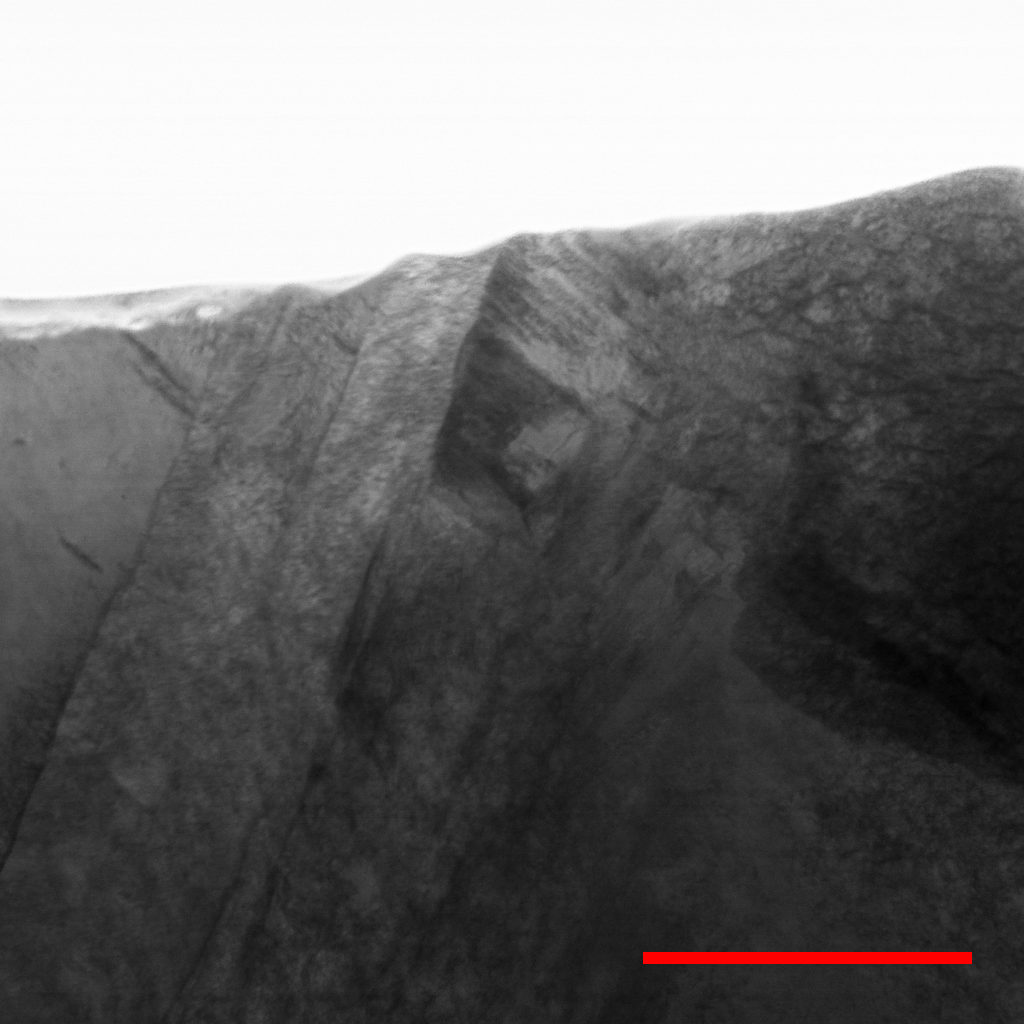
\includegraphics[scale=0.15]{../src/A1/1A-0036.png}};
    \begin{scope}[x={(image.south east)},y={(image.north west)}]
      \filldraw[fill=white,draw=white] (0.628,0.0615) rectangle node[above] {
          \footnotesize\color{\col}\SI{500}{\nano\metre}} +(0.32,0.015);
      \filldraw[fill=white,draw=black] 
        (0.01,0.89) rectangle +(0.1,0.1) node[pos=0.5] {\footnotesize (a)};
      %\node at (0.5,-0.1) {(a) STEM (BF) $\times$120k.};
    \end{scope}
  \end{tikzpicture}}
  \fbox{\begin{tikzpicture} 
    \node[anchor=south west,inner sep=0] (image) at (0,0) {
      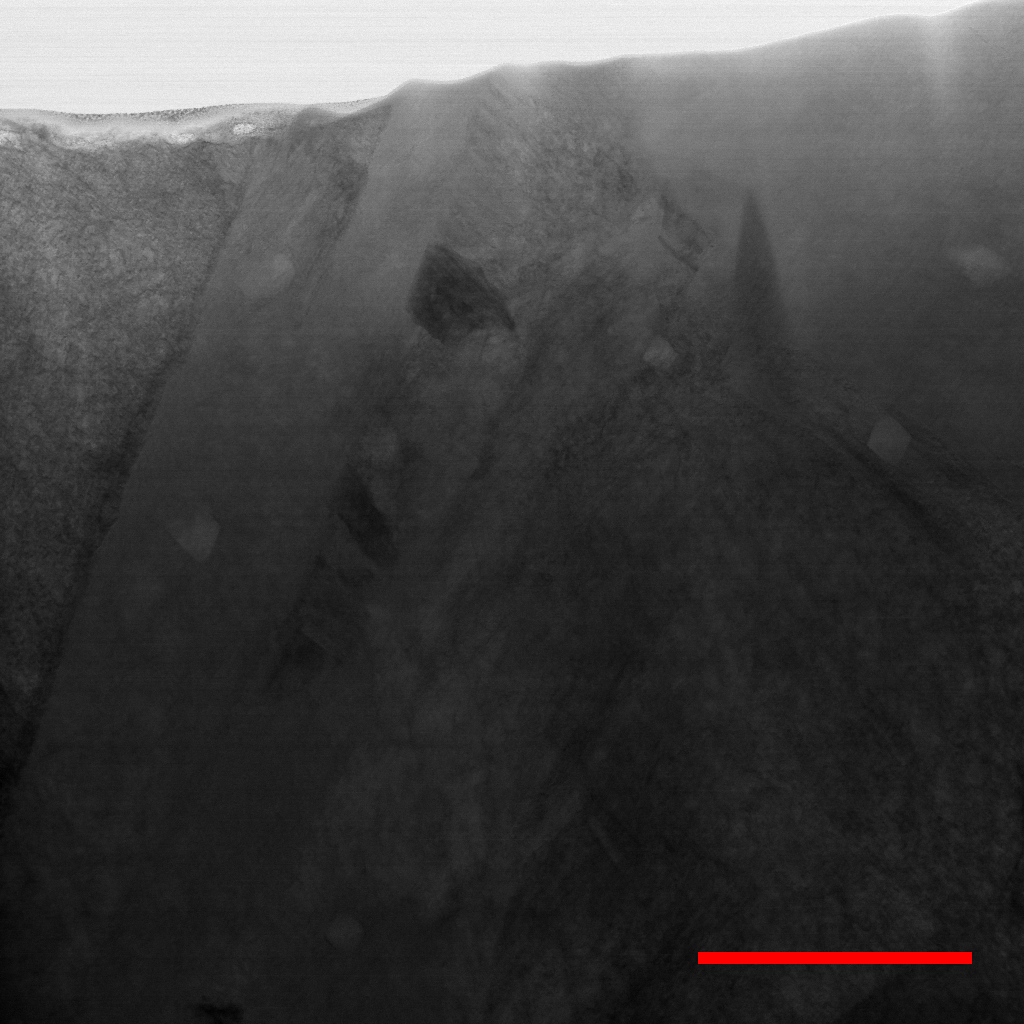
\includegraphics[scale=0.15]{../src/A1/1A-0022.png}};
    \begin{scope}[x={(image.south east)},y={(image.north west)}]
      \filldraw[fill=white,draw=white] (0.678,0.0615) rectangle node[above] {
        \footnotesize\color{\col}\SI{500}{\nano\metre}} +(0.27,0.015); 
      \filldraw[fill=white,draw=black] 
        (0.01,0.89) rectangle +(0.1,0.1) node[pos=0.5] {\footnotesize (b)};
      %\node at (0.5,-0.1) {(b) STEM (BF) $\times$100k.};
    \end{scope}
  \end{tikzpicture}}
\end{document}